\subsection{Raspberry Pi}

\begin{figure}[ht]
    \centering
    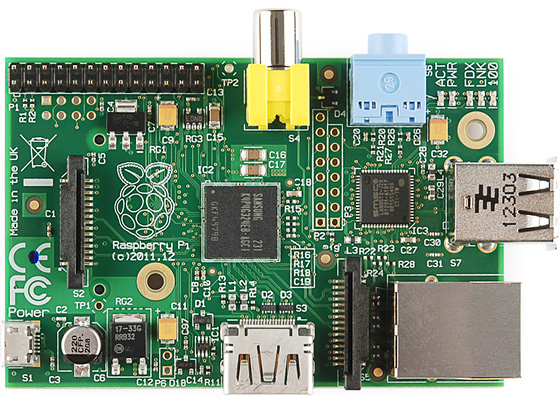
\includegraphics[scale=0.3]{images/raspberrypi}
    \caption{ \cite{img01} Raspberry Pi Modell B (oben)}
    \label{fig:raspberrypi}
\end{figure}
Das ausgew\"ahlte Modell B besitzt u.a. einen 700MHz Broadcom-Prozessor (ARM-Architektur), 500MB Arbeitsspeicher, 2 USB-2.0-Anschl\"usse sowie 17 frei programmierbare GPIO-Pins.
Auf dem Raspberry Pi wird Debian GNU/Linux einngesetzt.

\newpage

\subsection{Kamera}

\begin{figure}[ht]
    \centering
    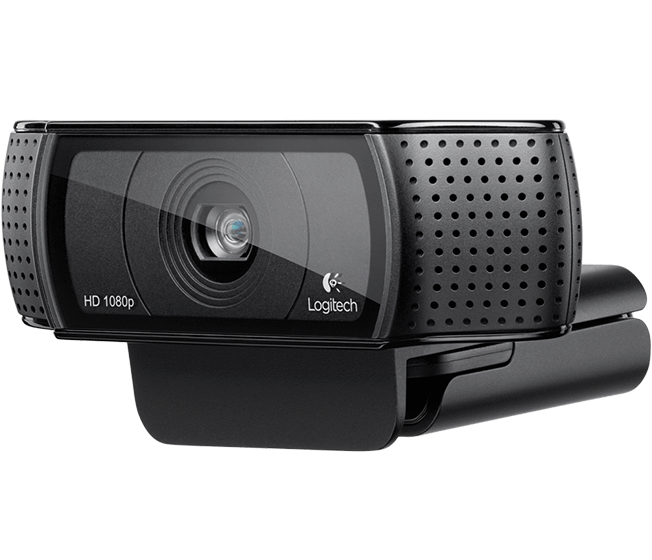
\includegraphics[scale=0.2]{images/c920webcam}
    \caption{\cite{img02} Logitech HD Pro Webcam C920}
    \label{fig:webcam}
\end{figure}
Als Kamera wird eine Logitech HD Pro Webcam C920 verwendet\footnote{\href{https://secure.logitech.com/en-us/product/hd-pro-webcam-c920}{https://secure.logitech.com/en-us/product/hd-pro-webcam-c920}}.
Die USB-Kamera unterst\"utzt Aufnahmen mit bis zu 1920x1080 Pixel bei 30 Bildern pro Sekunde bzw. 1280x720 Pixel bei 60 Bildern pro Sekunde. Integriert ist au{\ss}erdem ein H264-Hardware-Encoder, was bei diesem Projekt besonders von Vorteil ist, da die Rechenleistung des ausgew\"ahlten Raspberry Pi-Modells nicht ausreicht, um die Video-Daten effizient zu codieren.\\


\subsection{Netzteil}
Die \"ublichen 1200mA-Netzteile sind zu schwach, wenn eine Webcam angeschlossen werden soll, da diese zeitweise eventuell einen hohen Stromverbrauch hat.
\begin{figure}[h]
    \centering
    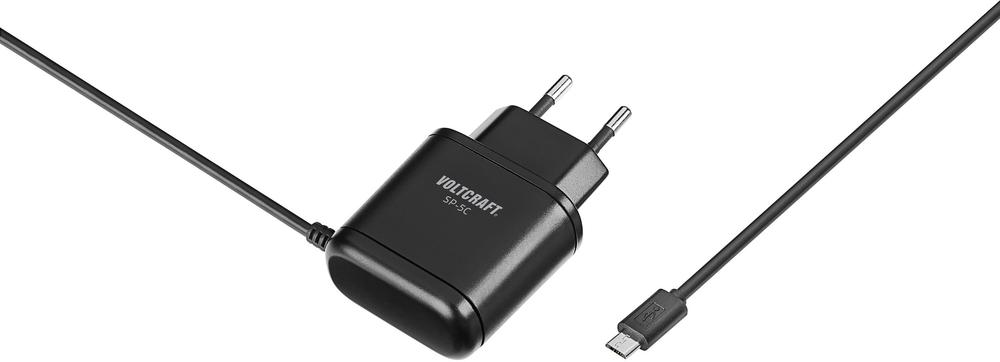
\includegraphics[scale=0.2]{images/netzteil}
    \caption{\cite{img03} Voltcraft SP-5C}
    \label{fig:netzteil}
\end{figure}
Daher wird f\"ur diesen Anwendungsfall ein \"uberlastungsgesch\"utztes 2500mA-USB-Netzteil\footnote{Das verwendete Netzteil ist ein Voltcraft SP-5C} verwendet.\\

\subsection{Sensor}
Der Sensor wird zur Erkennung des Zustands der T\"ur eingesetzt.
\begin{figure}[h]
    \centering
    \begin{subfigure}[t]{0.5\textwidth}
        \centering
        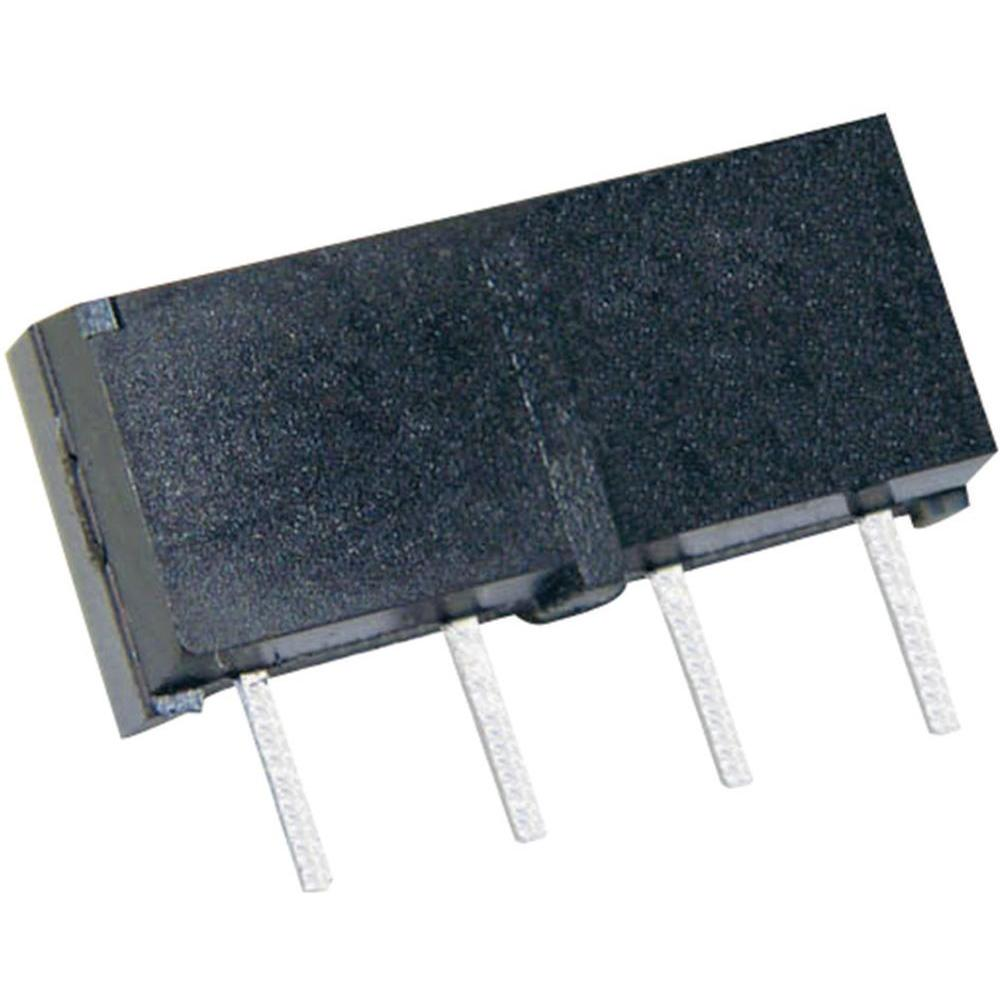
\includegraphics[scale=0.05]{images/sensor}
        \caption{\cite{img04} Reed-Kontakt}
    \end{subfigure}%
    \begin{subfigure}[t]{0.5\textwidth}
        \centering
        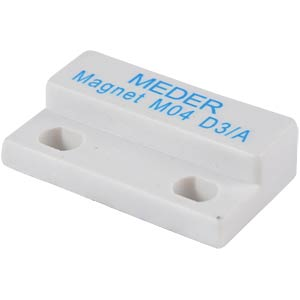
\includegraphics[scale=0.2]{images/MAGNET_M4}
        \caption{\cite{img05} Bet\"atigungsmagnet}
    \end{subfigure}
    \caption{Sensor und Magnet}
    \label{fig:sensor}
\end{figure}
\\Verwendet wird hier ein Reed-Kontakt\footnote{Genaue Bezeichnung des Bauteils: MS05-1A87-75DHR} mit passendem Bet\"atigungsmagnet.
Damit der Sensor besser befestigt werden kann wird er auf eine kupferbeschichtete Hartpapier-Platine gel\"otet. Au{\ss}erdem werden die Anschl\"usse auf eine Stiftleiste gef\"uhrt, um die Verbindung mit den GPIO-Pins des Raspberry Pi zu vereinfachen.\\

\subsection{Gesamtaufbau}
\begin{figure}[ht]
    \centering
    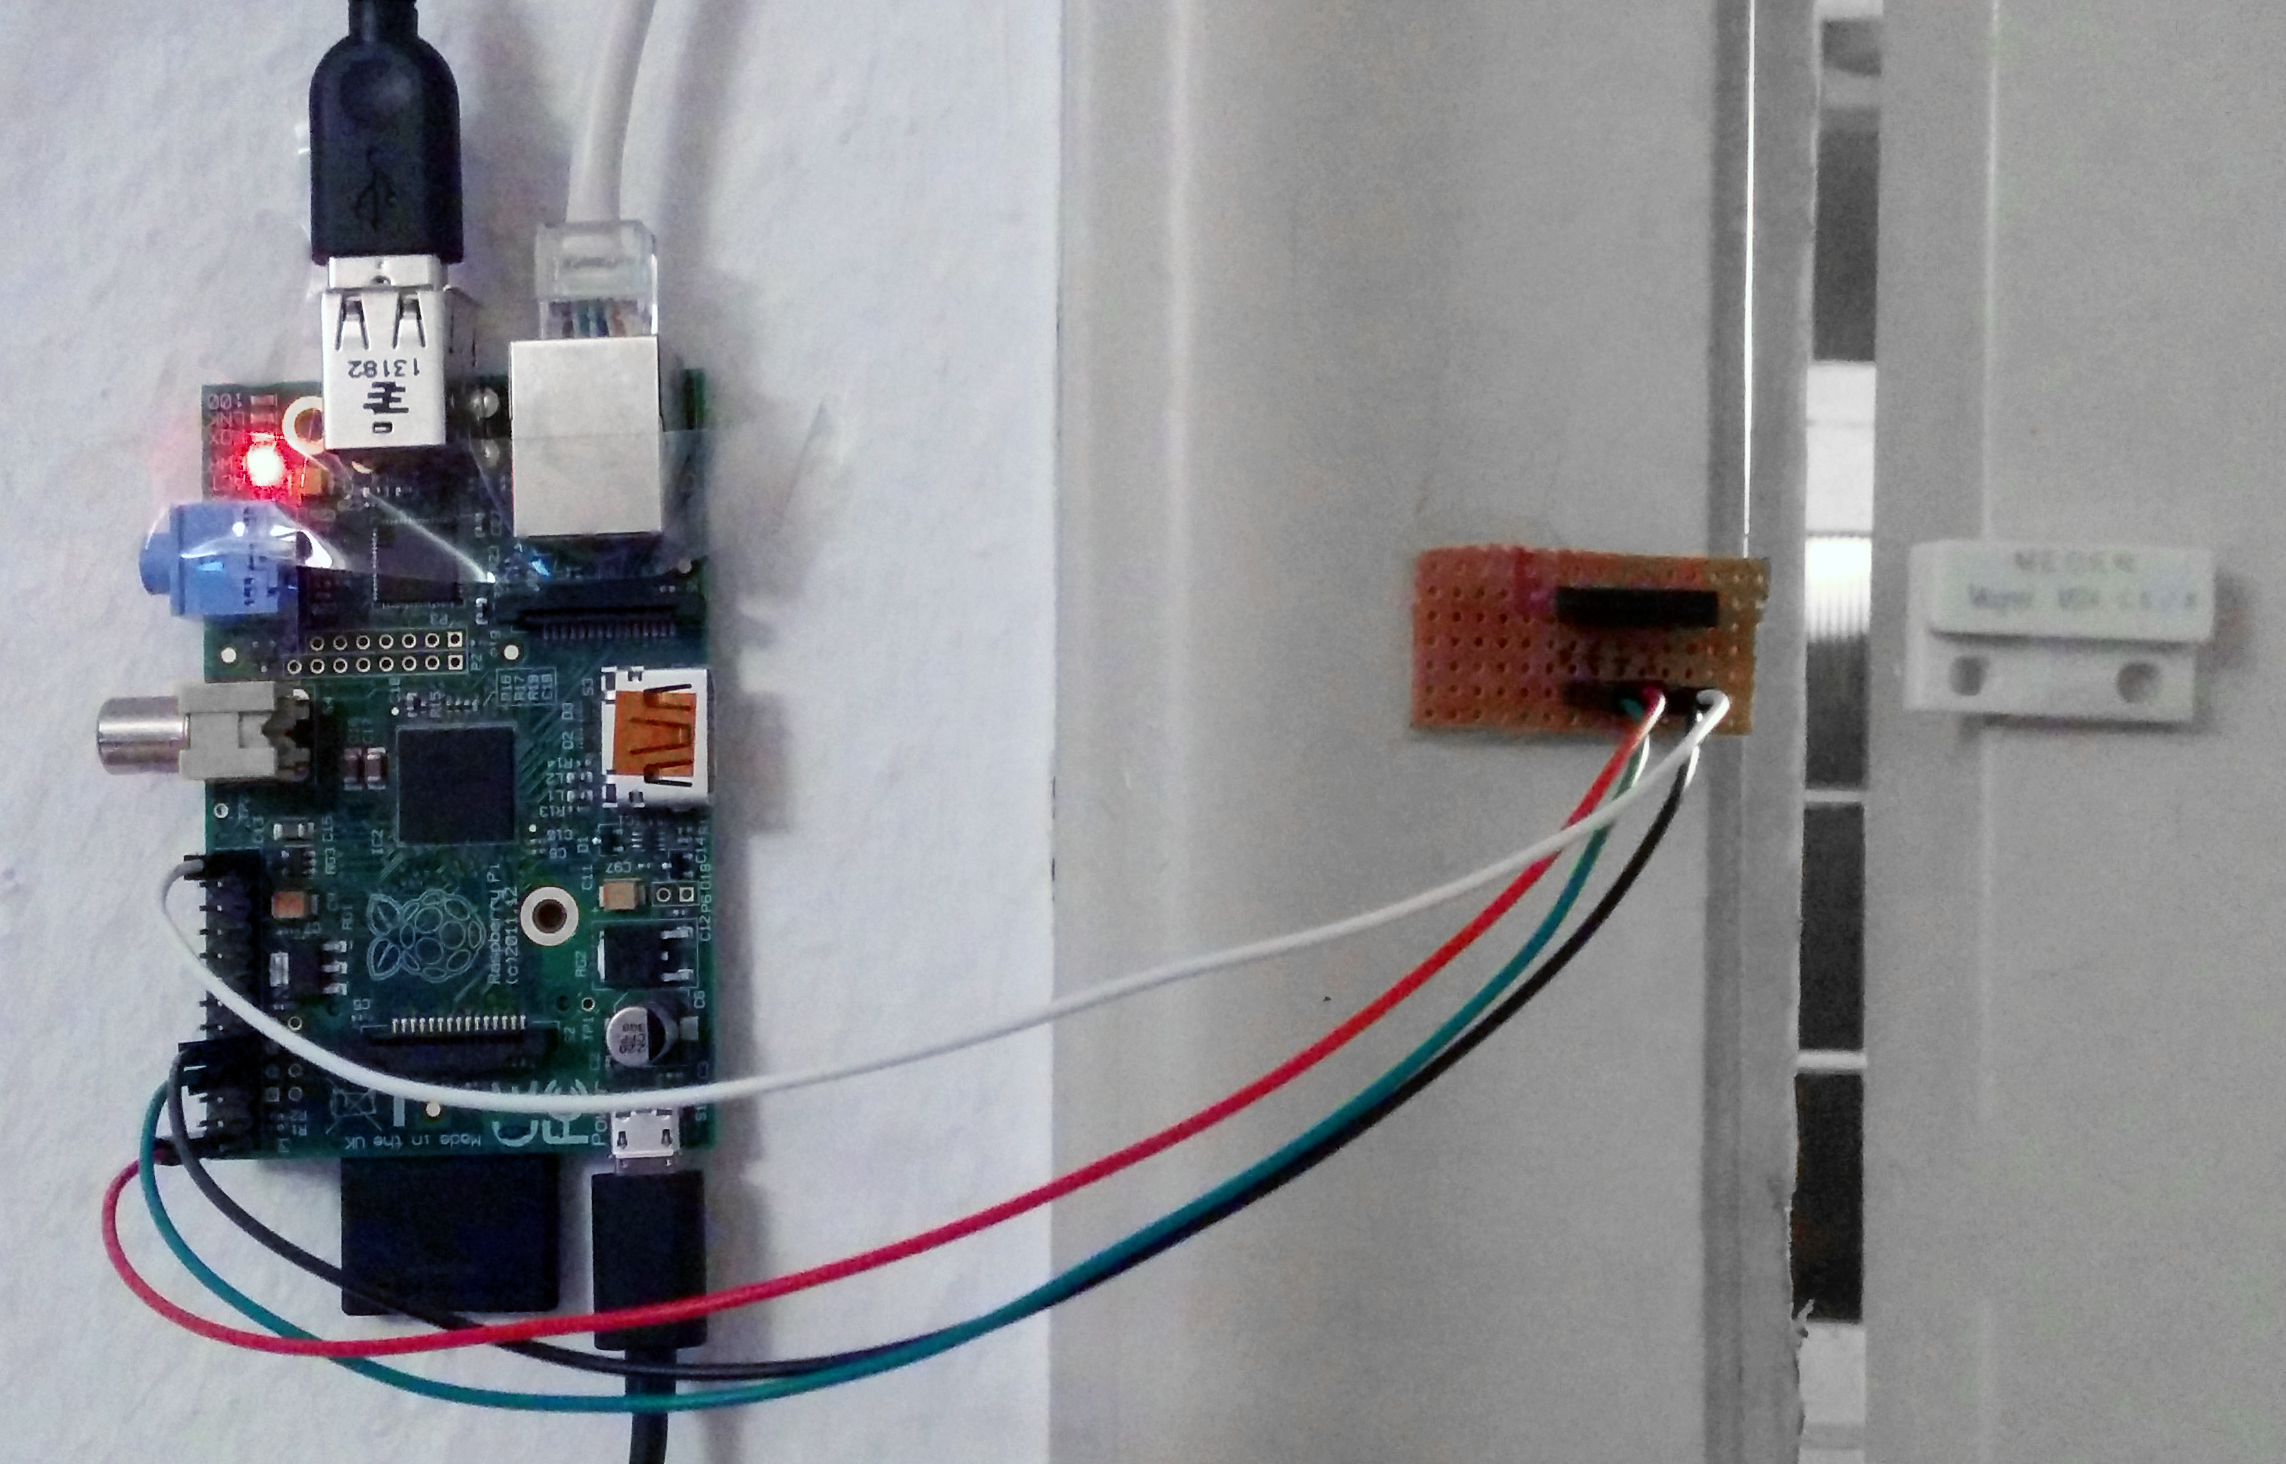
\includegraphics[scale=0.15]{images/aufbauklein}
    \caption{Gesamtaufbau der Hardware}
    \label{fig:gesamt}
\end{figure}

\newpage
